\scanpage{241}
\mspage{768}

\deleted{\unsure{(44)|(42)}}
\[
a\in\mathbb R^2\setminus\mathbb Z^2,
\]
\unsure{up} above $a_{1,1}$, we will thus have a canonical isomorphism
\[
\text{(42)}\qquad
\Pi_{1,1}\simeq\pi_1(\mathbb R^2\setminus\mathbb Z^2,\mathbb Z^2;a)
\]
whence an exact sequence
\diagram{\begin{tikzcd}[ampersand replacement=\&,column sep=small,row sep=small]
\text{(43)}\quad \& 1\arrow[r] \&
\pi_1(\mathbb R^2\setminus\mathbb Z^2)\arrow[r] \&
\Pi_{1,1}\arrow[r]\arrow[d,equal] \&
\mathbb Z^2\arrow[r]\arrow[d,phantom,"\simeq"{description,rotate=90}] \& 1.\\
\&\&\&\pi_1(U_{1,1}=X_1\setminus\{a_{1,0}\}) \&
\pi_1(X_1)\arrow[d,phantom,"\simeq"{description,rotate=90}] \&\\
\&\&\&\& (\Pi_{1,1})_{\mathrm{ab}} \&
\end{tikzcd}}

The elements of the mixed $\pi_1$ are made explicit by Jean Malgoire's calculation using the pairs
\[
\text{(44)}\qquad
(\gamma,\ell)\qquad
\left(\begin{gathered}
\gamma\in\mathbb Z^2,\quad \ell\ \text{\unsure{class} of paths in}\\
\mathbb R^2\setminus\mathbb Z^2\ \text{from }a\text{ to }\deleted{\unsure{\gamma|\tau}}a+\gamma
\end{gathered}\right)
\]
which we ``\unsure{compose} like functions''.

\inserted{We will take, over the generators}
\deleted{Let us consider the}
$e_0,e_1$ of $\mathbb Z^2$, the elements $x,y$ defined by the straight-line paths from $a$ to $a+e_0$, resp. $a+e_1$, starting from the origin
\[
\text{(45)}\qquad
 a=\widetilde a_{1,1}=\left(+\frac12,+\frac12\right)
\]

\figure{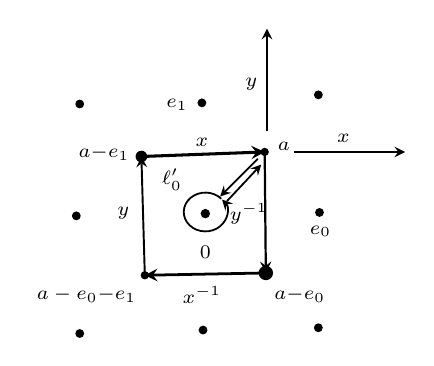
\begin{tikzpicture}[x=1.45cm,y=1.45cm,>=stealth,font=\scriptsize]
\fill (-1.10,0.96) circle (1.6pt);
\fill (-0.03,0.97) circle (1.6pt);
\fill (0.99,1.04) circle (1.6pt);
\fill (-1.13,-0.02) circle (1.6pt);
\fill (0,0) circle (1.7pt);
\fill (1.00,0.01) circle (1.6pt);
\fill (-1.10,-1.05) circle (1.6pt);
\fill (-0.02,-1.02) circle (1.6pt);
\fill (0.99,-1.00) circle (1.6pt);
\node[left] at (-0.07,0.95) {$e_1$};
\node[below] at (1.01,-0.02) {$e_0$};
\node[below] at (0,-0.20) {$0$};
\coordinate (a) at (0.52,0.54);
\coordinate (b) at (-0.56,0.50);
\coordinate (c) at (-0.53,-0.54);
\coordinate (d) at (0.53,-0.52);
\fill (a) circle (1.5pt);
\fill (b) circle (2.1pt);
\fill (c) circle (1.5pt);
\fill (d) circle (2.6pt);
\draw[->,line width=1.1pt] (b) -- (a);
\node[above] at (-0.03,0.50) {$x$};
\draw[->,line width=.7pt] (c) -- (b);
\node[left] at (-0.58,0.00) {$y$};
\draw[->,line width=1.0pt] (d) -- (c);
\node[below] at (-0.03,-0.55) {$x^{-1}$};
\draw[->,line width=.8pt] (a) -- (d);
\node at (0.38,0.00) {$y^{-1}$};
\draw[->,line width=.7pt] (0.54,0.72) -- (0.54,1.62);
\node[left] at (0.54,1.13) {$y$};
\draw[->,line width=.7pt] (0.78,0.54) -- (1.75,0.54);
\node[above] at (1.21,0.54) {$x$};
\node[right] at (0.55,0.59) {$a$};
\node[left] at (-0.58,0.53) {$a\unsure{-}e_1$};
\node[below left] at (-0.52,-0.56) {$a-e_0\unsure{-}e_1$};
\node[below right] at (0.52,-0.56) {$a\unsure{-}e_0$};
\draw[->,line width=.65pt] (0.46,0.48) -- (0.13,0.15);
\draw[->,line width=.65pt] (0.19,0.11) -- (0.49,0.43);
\draw[->,line width=.65pt] (0.14,0.13)
 arc[start angle=43,end angle=400,x radius=.19,y radius=.17];
\node[above left] at (-0.12,0.12) {$\ell'_0$};
\end{tikzpicture}}

Then the element $xyx^{-1}y^{-1}$ is represented by the path above, which is visibly opposite to the positively oriented ``straight-line'' loop from $a$ around the origin $0$.
\margin{240}

\begin{center}
240\\
\texttt{https://grothendieck.umontpellier.fr}\\
Université de Montpellier, UMR CNRS 5149, Case courrier 051, Place Eugène Bataillon\\
34095 Montpellier cedex 5 - France
\end{center}

\scanpage{242}

$5^\circ$) \uline{Digression on the} \inserted{\uline{coverings of}} \uline{germs of spaces.}

\margin{A) \uline{Coverings of germs}}
\margin{here we exclude \deleted{\unsure{the}} \inserted{not the} improper filter $(\varnothing\in\Phi)$ corresponding to the \uline{empty} germ of spaces}

A ``germ of spaces'' is defined by a topological space $S$ and a \deleted{base of a} filter $\Phi$ on $S$, a morphism from $(S,\Phi)$ to $(S',\Phi')$ is an element of
\[
\text{(46)}\qquad
\varinjlim_{S_i\in\Phi}\operatorname{Hom}_{\Phi_{\unsure{S_i|S'_i}},\Phi'}(S_i,S'),
\]
where \deleted{$\Phi_{S_i}$ is} for $S_i\in\Phi$, $\Phi_{S_i}$ is the filter induced by $\Phi$ on $S_i$, and $\operatorname{Hom}_{\Phi_{S_i},\Phi'}$ denotes the set of continuous maps \inserted{$f$} from $S_i$ to $S'$ compatible with $\Phi_{S_i},\Phi'$, i.e. such that $\forall S'_j\in\Phi'$, \deleted{$\unsure{f}$} we have $f^{-1}(S'_j)\in\Phi_{S_i}$. The composition of morphisms of germs is obvious.

A \uline{covering} (étale) of a germ $(S,\Phi)$ of topological spaces is an object of the category
\[
\text{(47)}\qquad
\underline{\mathrm{Rev}}(S,\Phi)=\varinjlim_{S_i\in\Phi}\underline{\mathrm{Rev}}(S_i);\qquad\unsure{*}
\]
\unsure{these|the} coverings form a category, which we could \inserted{probably} interpret \inserted{(at least in ``good cases'')} as the category of coverings of a suitable topos (namely the projective limit topos
\margin{241}

\begin{center}
241\\
\texttt{https://grothendieck.umontpellier.fr}\\
Université de Montpellier, UMR CNRS 5149, Case courrier 051, Place Eugène Bataillon\\
34095 Montpellier cedex 5 - France
\end{center}

\scanpage{243}
\mspage{769}

\margin{this \unsure{has been} done by Olivier Leroy?}

of the \inserted{(small)} étale topoi of the $S_i\in\Phi$).

This category, ``in the good cases'', tends to be multi-Galois, or even Galois.

We say that a germ \deleted{\unsure{is}} of spaces is $1$-connected, or simply connected, if the natural functor

\diagram{\begin{tikzcd}[ampersand replacement=\&,column sep=large,row sep=small]
{(48)} \& (\mathrm{Ens}) \arrow[r] \& \underline{\mathrm{Rev}}(S,\Phi) \\
 \& E \arrow[r,mapsto] \& {\unsure{{}^{1}\!E_{(S,\Phi)}|\widetilde E_{(S,\Phi)}},\ \text{constant covering with}} \\
 \& \& {\text{value }\unsure{E|\Phi}}
\end{tikzcd}}

is an equivalence of categories. This means that

$1^\circ)$ This functor is fully faithful (we say that $(S,\Phi)$ is $0$-connected), which means, if $S$ is locally connected, that $\forall S_i\in\Phi$, $\exists S_j\in\Phi$, $S_j\subset S_i$, such that \inserted{$S_j\ne\varnothing$ and} $(\pi_0(S_j)\longrightarrow\pi_0(S_i))$ is a constant map

\margin{thus this implies that this germ of spaces is nonempty}

$2^\circ)$ the functor is moreover \unsure{essentially!|essentially$^{\mathrm t}$} surjective, which means that for every $S_i\in\Phi$, $\exists S_j\in\Phi$, \inserted{$S_j\subset S_i$} such that for every connected component $S_{j,\alpha}$ of $S_j$, the outer homomorphism $\pi_1(S_{j,\alpha})\longrightarrow\pi_1(S_i)$ is trivial.

Coverings of germs of spaces form a fibered category over that

\margin{242}

\begin{center}
242\\
\texttt{https://grothendieck.umontpellier.fr}\\
Université de Montpellier, UMR CNRS 5149, Case courrier 051, Place Eugène Bataillon\\
34095 Montpellier cedex 5 - France
\end{center}

\scanpage{244}

of germs of spaces. The category of topological spaces \deleted{\illegible{1}} can be regarded as a full subcategory of that of germs of topological spaces by \unsure{associating} to every space $\unsure{S}$, the germ $(S,\Phi)$, where $\Phi$ is the trivial filter on $S$. This being so, the fibered category of coverings of germs of spaces \unsure{induces|induced} that of coverings of topological spaces.

Let $\deleted{\unsure{\mathcal S}}\mathcal X$ be a germ of spaces such that $\underline{\mathrm{Rev}}\mathcal X$ is a \inserted{multi-}Galois category, \deleted{Then} and let $\mathcal S$ be a $1$-connected germ of spaces, $\mathcal S\longrightarrow\mathcal X$ a morphism. Then we have

\diagram{\begin{tikzcd}[ampersand replacement=\&,column sep=large]
{(49)} \& \underline{\mathrm{Rev}}(\mathcal X) \arrow[r] \& \underline{\mathrm{Rev}}(\mathcal S) \& (\mathrm{Ens}) \arrow[l,"\sim"']
\end{tikzcd}}

fiber functor on $\underline{\mathrm{Rev}}(\mathcal X)$, which makes it possible to define
\[
(50)\qquad \pi_1(\deleted{\unsure{\mathcal S}}\unsure{\mathcal X},\mathcal S)
\]
as the $\pi_1$ relative to this fiber functor. If $\mathcal X$ is $0$-connected so $\underline{\mathrm{Rev}}(\mathcal X)$ is Galois, we will thus have, if $\Pi\simeq\pi_1(\mathcal X,\mathcal S)$, an equivalence of categories

\margin{243}

\begin{center}
243\\
\texttt{https://grothendieck.umontpellier.fr}\\
Université de Montpellier, UMR CNRS 5149, Case courrier 051, Place Eugène Bataillon\\
34095 Montpellier cedex 5 - France
\end{center}

\scanpage{245}
\mspage{770}

\[
(51)\qquad \underline{\mathrm{Rev}}(\mathcal X)\simeq\mathrm{Ens}(\Pi).
\]

The group $\pi_1(\mathcal X,\mathcal S)$ depends functorially on the triple $(\mathcal S,\mathcal X,\mathcal S\longrightarrow\mathcal X)$ i.e. on the arrow $\mathcal S\longrightarrow\mathcal X$ in the category of germs of spaces, where $\deleted{\mathcal S}$ the source $\mathcal S$ is $1$-connected.

\unsure{Let|Let} $X$ be a topological space, $Y$ a subset of $X$, we \uline{call the germ of} $X$ \uline{around} $Y$ the germ of spaces $(X,\Phi)$, where $\Phi$ is the filter of neighborhoods of $Y$ \unsure{in|in} $X$, \uline{the residual germ of $X$ around $Y$} the germ of spaces $(X\setminus Y,\Phi_{X\setminus Y})$ induced on $X-Y$ (it is empty iff $Y$ is open).

\margin{We have a \unsure{diagram} of \unsure{canonical} morphisms
\diagram{\begin{tikzcd}[ampersand replacement=\&,column sep=large,row sep=large]
\unsure{\mathrm{Germ}_{Y}(X)} \arrow[d,hook] \& \unsure{\mathrm{Gerres}_{Y}(X)} \arrow[l,hook'] \arrow[d,hook] \\
X \& X-Y \arrow[l,hook']
\end{tikzcd}}\quad (52)}

We will use this notion \deleted{\unsure{especially}} in the case where $Y=\{x\}$, speaking also of the germ and residual germ of $X$ at $x$. (\uline{N.B.} the germ of $X$ at $x$ is always \deleted{\unsure{simp}} $1$-connected, but not the residual germ). Every germ of spaces \inserted{$(S,\Phi)$} can be interpreted as the residual germ of a space \deleted{$(\unsure{S},\unsure{\Phi})$} $\unsure{X}=S\cup\{\omega\}$ at a suitable point $\omega$ \ldots

\margin{244}

\begin{center}
244\\
\texttt{https://grothendieck.umontpellier.fr}\\
Université de Montpellier, UMR CNRS 5149, Case courrier 051, Place Eugène Bataillon\\
34095 Montpellier cedex 5 - France
\end{center}

\scanpage{246}

\unsure{.} I am interested in the case where $x\in X$ has a neighborhood homeomorphic to $\mathbb R^2$ --- i.e. $X$ is a surface at $x$. I will denote by $\deleted{D_{X,x}^{*}}$
\[
(53)\qquad D_{X,x}^{*}\quad\text{or}\quad D_x^{*}
\]
the residual germ of $X$ at $x$ (contained in the germ $D_{X,x}$ or $D_x$ of $X$ at $x$).

I am interested in the choice of a \uline{universal covering} $D_x^{*\,\sim}$ of $D_x^{*}$ --- but for \unsure{which|whom} I have to make a digression on the abstract notion of \uline{universal covering of a germ of spaces}.

Let $(S,\Phi)$ be a germ of spaces. A covering of $(S,\Phi)$ comes from a covering $S'_i$ of an $S_i\in\Phi$, and defines a germ of spaces $(S'_i,\Phi_{S'_i})$, where $\Phi_{S'_i}$ denotes the inverse image of $\Phi_{\deleted{\unsure{S'_i}}S_i}$ in $S'_i$. This germ of spaces \inserted{over $\mathcal S=(S,\Phi)$} (up to unique isomorphism of germs) does not depend on the choice of $S_i$, $S'_i$, but only on the element of $\underline{\mathrm{Rev}}(\mathcal S)$. We thus find a canonical functor

\margin{245}

\begin{center}
245\\
\texttt{https://grothendieck.umontpellier.fr}\\
Université de Montpellier, UMR CNRS 5149, Case courrier 051, Place Eugène Bataillon\\
34095 Montpellier cedex 5 - France
\end{center}

\scanpage{247}
\mspage{771}

\diagram{\begin{tikzcd}[ampersand replacement=\&,column sep=large]
{(54)} \& \underline{\mathrm{Rev}}(\mathcal S) \arrow[r] \& {(\unsure{\mathrm{Germesp}})/\mathcal S}
\end{tikzcd}}

which is \uline{fully faithful}. A germ of spaces $\mathcal S'$ over $\mathcal S$ is called \deleted{\unsure{the}} an \uline{étale covering} \uline{of} $\mathcal S$, if it is in the essential image. Thus the category $\underline{\mathrm{Rev}}(\mathcal S)$ of étale coverings of the germ of spaces $\mathcal S$ is equivalent to the full subcategory of the \deleted{\unsure{g}} category of germs of spaces, over the germ $\mathcal S$, \deleted{which} formed by the étale coverings of the said germ $\mathcal S$.

Let us assume \deleted{that} \unsure{always|always} that the category $\underline{\mathrm{Rev}}(\mathcal S)$ is \deleted{\unsure{g}} multi-Galois. The $1$-connected objects are called universal coverings of $\mathcal S$ --- \deleted{if $\underline{\mathrm{Rev}}(\mathcal S)$ is Galois,} they form a groupoid, connected iff $\underline{\mathrm{Rev}}(\mathcal S)$ is Galois i.e. iff the germ $\mathcal S$ is $0$-connected. The universal \unsure{coverings!|coverings} of $\mathcal S$ can be interpreted as germs of spaces. Let $\widetilde{\mathcal S}$ be such a universal covering, then $\widetilde{\mathcal S}$ is indeed a \unsure{$1$-connected|$1$. connected} germ of spaces, and $\widetilde{\mathcal S}\longrightarrow\mathcal S$ makes it possible to define $\pi_1(\mathcal S,\widetilde{\mathcal S})$. This being so, we have a canonical isomorphism
\[
(55)\qquad \pi_1(\mathcal S,\widetilde{\mathcal S})\simeq\mathrm{Aut}_{\underline{\mathrm{Rev}}(\mathcal S)}(\widetilde{\mathcal S})
\]

\margin{Which expresses that $\pi_1(\mathcal S,\widetilde{\mathcal S})$ is none other than the $\pi_1$ of the ``abstract'' \inserted{multi-}Galois category $\underline{\mathrm{Rev}}(\mathcal S)$, ``calculated'' at the $1$-connected element $\widetilde{\mathcal S}$.}

\margin{\figure{\begin{tikzpicture}[x=1cm,y=1cm]
\draw (0,0) -- (0.18,0.43);
\draw (0.04,0.10) -- (0.14,0);
\end{tikzpicture}}}

\margin{246}

\begin{center}
246\\
\texttt{https://grothendieck.umontpellier.fr}\\
Université de Montpellier, UMR CNRS 5149, Case courrier 051, Place Eugène Bataillon\\
34095 Montpellier cedex 5 - France
\end{center}